\documentclass[12pt]{article}

\usepackage[english]{babel}
\usepackage[utf8]{inputenc}
\usepackage{fancyhdr}

\usepackage[margin=1in]{geometry}
\usepackage{pgf}
\usepackage{pgfplots}
\usepackage{siunitx}
\usepackage{tikz}
\usepackage{float}
\usepackage{amsmath}

\usepackage[font=small,labelfont=bf]{caption}
\usepackage{pstricks-add}
\usepackage{pgfplotstable}
\usepackage{filecontents}
\usepackage{pgfplotstable}

\usetikzlibrary{scopes}
\usetikzlibrary{angles,quotes}
\usetikzlibrary{calc}
\pgfplotsset{compat=1.5}

\newcommand*{\I}{\imath}
\newcommand*{\J}{\jmath}
\newcommand{\norm}[1]{\lvert #1 \rvert}

\begin{filecontents}{data1.csv}
      E	    Y
    0	    0
    8000	0.04
    16000	0.07
    24000	0.11
    32000	0.14
    40000	0.17
    48000	0.21
    56000	0.24
    64000	0.27
    72000	0.31
    };
\end{filecontents}

\begin{document}
\sisetup{per-mode=symbol}

\begin{titlepage}
    \begin{center}
        \vspace*{1cm}
        \textbf{Motion of a Point Charge in a Uniform Electric Field}

        \vspace{0.5cm}
        Lab: 02

        \vspace{1cm}

        \textbf{Jaden Moore}

        \vfill

        Orange Coast College\\
        Physics A280L\\
        March 1st, 2021

    \end{center}
\end{titlepage}

\pagestyle{fancy}
\fancyhf{}
\setlength{\headheight}{15pt}
\lhead{Motion of a Point Charge in a Uniform Electric Field}
\rhead{Lab: 02}
\cfoot{\thepage}

\section{Introduction}
In this lab, we consider the motion of a point charge as it travels with some initial velocity $\vec{v_0}$ through a region of space occupied by an electric field $\vec{E}$. We first analyze the mass of the point charge and then in the second half, we consider the vertical displacement of the point charge caused by the electric field over time and compare the experimental displacement with the theoretical to find the percent error.

\section{The mass of the point charge}
Consider a point charge $+q$ positioned 70 cm away from a 100 cm long electric field $\vec{E}$. At $t=0$, the point charge is released with a velocity $\vec{V_0}=\SI{35}{cm/s}$. As $+q$ enters the electric field, the positive point charge attracts to the negative portion of the electric field and its y-position increases by some distance $\Delta y$.
\setlength{\tabcolsep}{1pt}
\renewcommand{\arraystretch}{1}
\newcolumntype{P}[1]{>{\centering\arraybackslash}p{#1}}

\begin{figure}[H]
    \centering

    \caption[10pt]{A point charge $+q$ positioned 70 cm from an electric field $\vec{E}$}

    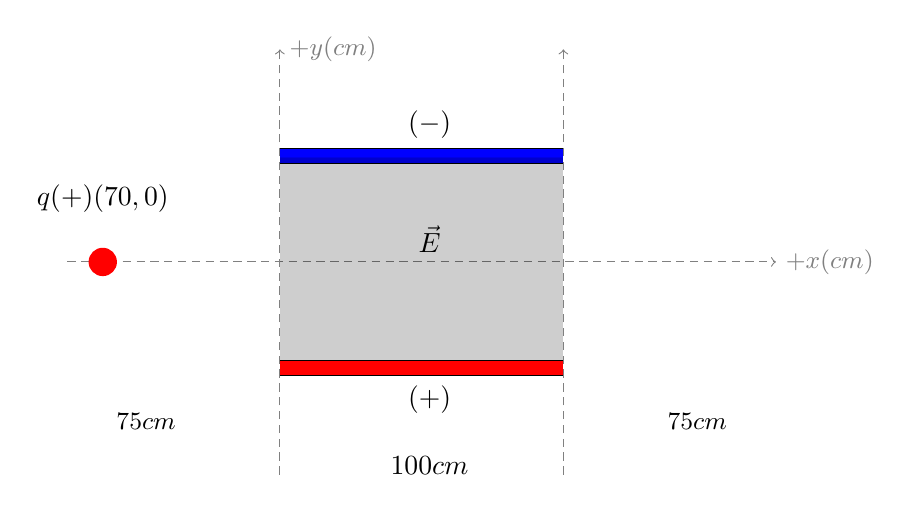
\begin{tikzpicture}[scale=0.9]
        \begin{scope}

            \draw[densely dashed,gray,font=\small,->] (-5, 1) -- (5,1) node[right] {$+x (cm)$};
            \draw[densely dashed,gray,font=\small,->, name=A] (-2,-2) -- (-2,4) node[right] {$+y (cm)$} node[below, shift={(-1.7,-4.5)}, black] {$75cm$};

            \draw[densely dashed,gray,font=\small,->, name=B] (2,-2) -- (2,4) node[below, shift={(1.7,-4.5)}, black] {$75cm$};


            \draw[double=blue, opacity=1, double distance=5] (-2,2.5) -- (2,2.5) node[above, shift={(-1.7,0.1)}] {$(-)$};
            \draw[double=black, opacity=0.1, double distance=75] (-2,1) -- (2,1) node[above, shift={(-1.7,0)}, black, opacity=1] {$\vec{E}$};
            \draw[double=red, opacity=1, double distance=5] (-2,-0.5) -- (2,-0.5) node[below, shift={(-1.7,-0.1)}] {$(+)$} node[below, shift={(-1.7,-1)}] {$100cm$};



            \fill[red] (-4.5,1) circle (2mm) node[above, shift={(0,0.5)}, black]{$q(+) (70, 0)$};


        \end{scope}
    \end{tikzpicture}
\end{figure}

\subsection{Data}
Below we put into a table the data collected by measuring the $\Delta y$ of the point charge caused by various values of the electric field. In order to collect this data, we use the Physlet\textregistered \space Physics: Practical Uses of Charges and Electric Fields simulation 23.4 and measure the displacement with a mouse.

\setlength{\tabcolsep}{3pt}
\renewcommand{\arraystretch}{1.1}

\begin{figure}[H]
    \begin{center}
        \begin{tabular}{ P{3cm} P{3cm} P{3cm} P{3cm} }
            \hline
            \multicolumn{4}{c}{Table 1: The vertical displacement $\Delta y$ as $\vec{E}$ increases} \\
            \hline
            E $[N/C]$ & E [x$10^4 N/C$] & $\Delta y [cm]$ & $\Delta y [m]$                           \\
            \hline
            0         & 0               & 0               & 0                                        \\
            8000      & 0.8             & 4               & 0.04                                     \\
            16000     & 1.6             & 7               & 0.07                                     \\
            24000     & 2.4             & 10              & 0.1                                      \\
            32000     & 3.2             & 14              & 0.14                                     \\
            40000     & 4               & 17              & 0.17                                     \\
            48000     & 4.8             & 21              & 0.21                                     \\
            56000     & 5.6             & 24              & 0.24                                     \\
            64000     & 6.4             & 27              & 0.27                                     \\
            72000     & 7.2             & 31              & 0.31                                     \\

            \hline
        \end{tabular}
    \end{center}
\end{figure}

\subsection{Data Analysis}
A preliminary analysis of the data indicates that as the electric field $\vec{E}$ increases, the y-axis displacement of the point charge increases. This ultimately concludes that the displacement $\Delta y$ scales linearly with the strength of the electric field.

\subsection{Graph}
Now consider the data gathered in Table 1 in the form of a linear regression line graphed below.

\begin{figure}[H]
    \centering

    \caption[10pt]{Force exerted on a point charge over distance}

    \begin{tikzpicture}
        \pgfplotsset{width=10cm,
            legend style={font=\footnotesize}}
        \begin{axis}[
                xlabel={E $[N/C]$},
                xmin=0,
                xmax=80000,
                ylabel={$\Delta y[m]$},
                ymin=0,
                ymax=0.45,
                scaled x ticks=base 10:-3,
                yticklabel={\pgfmathprintnumber{\tick}},
                xticklabel={\pgfmathprintnumber{\tick}k},
                legend cell align = left,
                legend pos = north east,
            ]
            \addplot[only marks] table[x=E,y=Y]{data1.csv};
            \addplot[black,smooth,domain=0:72000] {4.23*10^(-6)*x + 3.82*10^(-3)};
            \addlegendimage{only marks}
            \addlegendentry{data point}
            \addlegendimage{no markers, red}
            \addlegendentry{$\Delta y=4.23x10^{-6}(E) + 3.82x10^{-3}$}
        \end{axis}
    \end{tikzpicture}
\end{figure}

\subsection{Graph Analysis}
An analysis of the graph indicates that as the electric field increases, the displacement of the point charge in the y-direction increases. From the linear regression we get the general equation of the line of best fit to be:

\begin{equation} \label{eq1}
    \Delta y=4.23x10^{-6}E + 3.82x10^{-3}
\end{equation}

Therefore, the slope of the line of best fit is $\SI{4.23}{x10^{-6}\metre\coulomb\per\newton}$. Utilizing the value of the slope we are able to calculate the mass of the point charge using the following formula as such:

\begin{equation} \label{eq2}
    m = \frac{q(\Delta t_1)^2}{2(slope)} = \frac{(10^{-8}C)(2.857s)^2}{2(\SI{4.23}{x10^{-6}\metre\coulomb\per\newton})} = \SI{0.00966}{kg} = \SI{9.66}{g}
\end{equation}

Where $q=10^{-6}C$, Coulomb's constant and $\Delta t_1=2.857s$, the time it takes the point charge to travel through the electric field at 35 cm/s.

\section{The position of the point charge}
We can calculate the y-position of the point charge at the end of the animation using the following formula as such:

\begin{equation} \label{eq3}
    \begin{split}
        y_{theory} & = \frac{qE(\Delta t_1)}{m}\left[\frac{\Delta t_1}{2} + \Delta t_2\right] \\
        & =\frac{(10^{-8}C)(\SI{0.8}{x10^4\newton\per\coulomb})(2.857s)}{\SI{0.00966}{kg}}\left[\frac{2.857s}{2} + 2.0s\right] \\
        & = 0.0812 m \\
        y_{theory} & = 8.12 cm
    \end{split}
\end{equation}

Where $\Delta t_2$ = 2.0s, the time at which the point charge enters the electric field, and $m$ = $\SI{9.66}{g}$, the mass of the point charge. We also let $\vec{E}=\SI{0.8}{x10^4\newton\per\coulomb}$ as an example calculation.
Now we put the calculations from Equation 3 in the form of a table below along with the corresponding percent error between $y_{theory}$ and $y_{exp}$ as such:

\setlength{\tabcolsep}{3pt}
\renewcommand{\arraystretch}{1.1}

\begin{figure}[H]
    \begin{center}
        \begin{tabular}{ P{3cm} P{3cm} P{3cm} P{3cm} }
            \hline
            \multicolumn{4}{c}{Table 2: The vertical displacement $\Delta y$ at different values of $\vec{E}$} \\
            \hline
            $\vec{E}$ [x$10^4 N/C$] & $y_{exp}[cm]$ & $y_{theory}$ [cm] & $\%$ error                         \\
            \hline
            0.8             & 8.0           & 8.12              & 1.47                               \\
            1.6             & 16.5          & 16.25             & 1.51                               \\
            2.4             & 25.0          & 24.38             & 2.5                                \\
            3.2             & 33.0          & 32.50             & 2.2                                \\
            \hline
        \end{tabular}
    \end{center}
\end{figure}

We notice that the y-displacement of the point charge gathered during the experiment was within 3\% margin of error with respect to the theoretical value.

\section{Conclusion}
It appears that as the strength of an electric field increases, the displacement of the point charge traveling through it increases. In the experiment, we were able to prove this by measuring the displacement $\Delta y$ on the point charge $q$ for different values of the electric field $\vec{E}$. We noticed that as $\vec{E}$ increased, the displacement $\Delta y$ increased at a linear rate. Using a linear regression model, we found the rate of change to be $\SI{4.23}{x10^{-6}\metre\coulomb\per\newton}$. Using this value, we were able to calculate the mass of the point charge and then subsequently predict the displacement of the point charge caused by the electric field. These predictions yielded a percent error of less than 3\% which indicates that our predictions were accurate.

The greatest obstacle in the lab was ensuring the units of each value used was correct and understanding how they interact. The biggest takeaway is further understanding how a point charge moves in response to the effects of an electric field and at what rate depending on the strength of the field.
\end{document}
